\documentclass[conference]{IEEEtran}
\IEEEoverridecommandlockouts
% The preceding line is only needed to identify funding in the first footnote. If that is unneeded, please comment it out.
%Template version as of 6/27/2024

\usepackage{cite}
\usepackage{amsmath,amssymb,amsfonts}
\usepackage{algorithmic}
\usepackage{graphicx}
\usepackage{textcomp}
\usepackage{xcolor}
\def\BibTeX{{\rm B\kern-.05em{\sc i\kern-.025em b}\kern-.08em
    T\kern-.1667em\lower.7ex\hbox{E}\kern-.125emX}}
    

\definecolor{dg}{RGB}{64,64,64}

\usepackage[colorlinks = true,
		citecolor = blue,
		urlcolor= blue,
		linkcolor=dg,]{hyperref}

\begin{document}

\title{Evaluating Progress in Web3 Grants: Introducing the Grant Maturity Index.
\thanks{This work is has been funded by the EU in the framework of the NGI TRUSTCHAIN project under the European Commission HORIZON-CL4-2022-HUMAN-01-03 grant: \href{https://cordis.europa.eu/project/id/101093274}{101093274} and by \href{https://ens.domains/}{ENS Domains} through its \textit{Large Grants} program.}
}
\author{\IEEEauthorblockN{1\textsuperscript{st} Ben Biedermann}
\IEEEauthorblockA{\textit{Islands and Small States Institute} \\
\textit{University of Malta}\\
Msida, Malta \\
\href{https://orcid.org/0000-0003-1331-6517}{0000-0003-1331-6517}}

\and
\IEEEauthorblockN{2\textsuperscript{nd} Fahima Gibrel}
\IEEEauthorblockA{\textit{Grant Innovation Lab} \\
\textit{Metagovernance Project Inc}\\
Brookline (MA), United States \\
\href{mailto:mgibrel.fahima@gmail.com}{gibrel.fahima@gmail.com}}

\and
\IEEEauthorblockN{3\textsuperscript{rd} Victoria Kozlova}
\IEEEauthorblockA{\textit{WID3\textsuperscript{+}} \\
\textit{acurraent UG} \\
Frankfurt (Oder), Germany \\
\href{https://orcid.org/0000-0003-3303-3143}{0000-0003-3303-3143}}
}
\maketitle

\begin{abstract}
This report introduces the Grant Maturity Index (GMI), a novel evaluative framework designed to assess the maturity and operational effectiveness of Web3 grant programs. As Web3 continues to develop, the decentralized nature of these programs brings both opportunities and challenges, particularly when it comes to governance, transparency, and community engagement. Traditional funding models are often governed by standardized processes, but Web3 grants lack such consistency, making it difficult for grant operators to measure the long-term success of their programs.

The \textit{Grant Maturity Index (GMI)} was created through \textit{exploratory applied research} to address this gap. Inspired by the World Bank’s GovTech Maturity Index (GTMI), the GMI is tailored specifically for the decentralized Web3 ecosystem. The GMI evaluates key dimensions of grant programs—governance, transparency, operational efficiency, and community engagement -- providing grant operators with a clear benchmark for assessing and improving their programs.

The primary objectives of this research are to:
\begin{itemize}
    \item Identify the structural indicators that adequately describe Web3 grant programs.
    \item Describe optimal outcomes for programs by evaluating their maturity across key operational areas.
\end{itemize}

In this report, the GMI is applied to four major Ethereum Layer 2 grant programs -- \textit{Arbitrum}, \textit{Mantle}, \textit{Taiko Labs}, and \textit{Optimism}. These case studies highlight areas where Web3 grant programs require improvement, particularly in \textit{standardizing processes}, enhancing \textit{transparency}, and increasing \textit{community participation}.
\end{abstract}

\begin{IEEEkeywords}
maturity model, Web3 governance, decentralised autonomous organisations, crypto-economic systems, mixed-methods
\end{IEEEkeywords}

\section{Introduction}


\begin{table}[htbp]
\caption{Table Type Styles}
\begin{center}
\begin{tabular}{|c|c|c|c|}
\hline
\textbf{Table}&\multicolumn{3}{|c|}{\textbf{Table Column Head}} \\
\cline{2-4} 
\textbf{Head} & \textbf{\textit{Table column subhead}}& \textbf{\textit{Subhead}}& \textbf{\textit{Subhead}} \\
\hline
copy& More table copy$^{\mathrm{a}}$& &  \\
\hline
\multicolumn{4}{l}{$^{\mathrm{a}}$Sample of a Table footnote.}
\end{tabular}
\label{tab1}
\end{center}
\end{table}

\begin{figure}[htbp]
\centerline{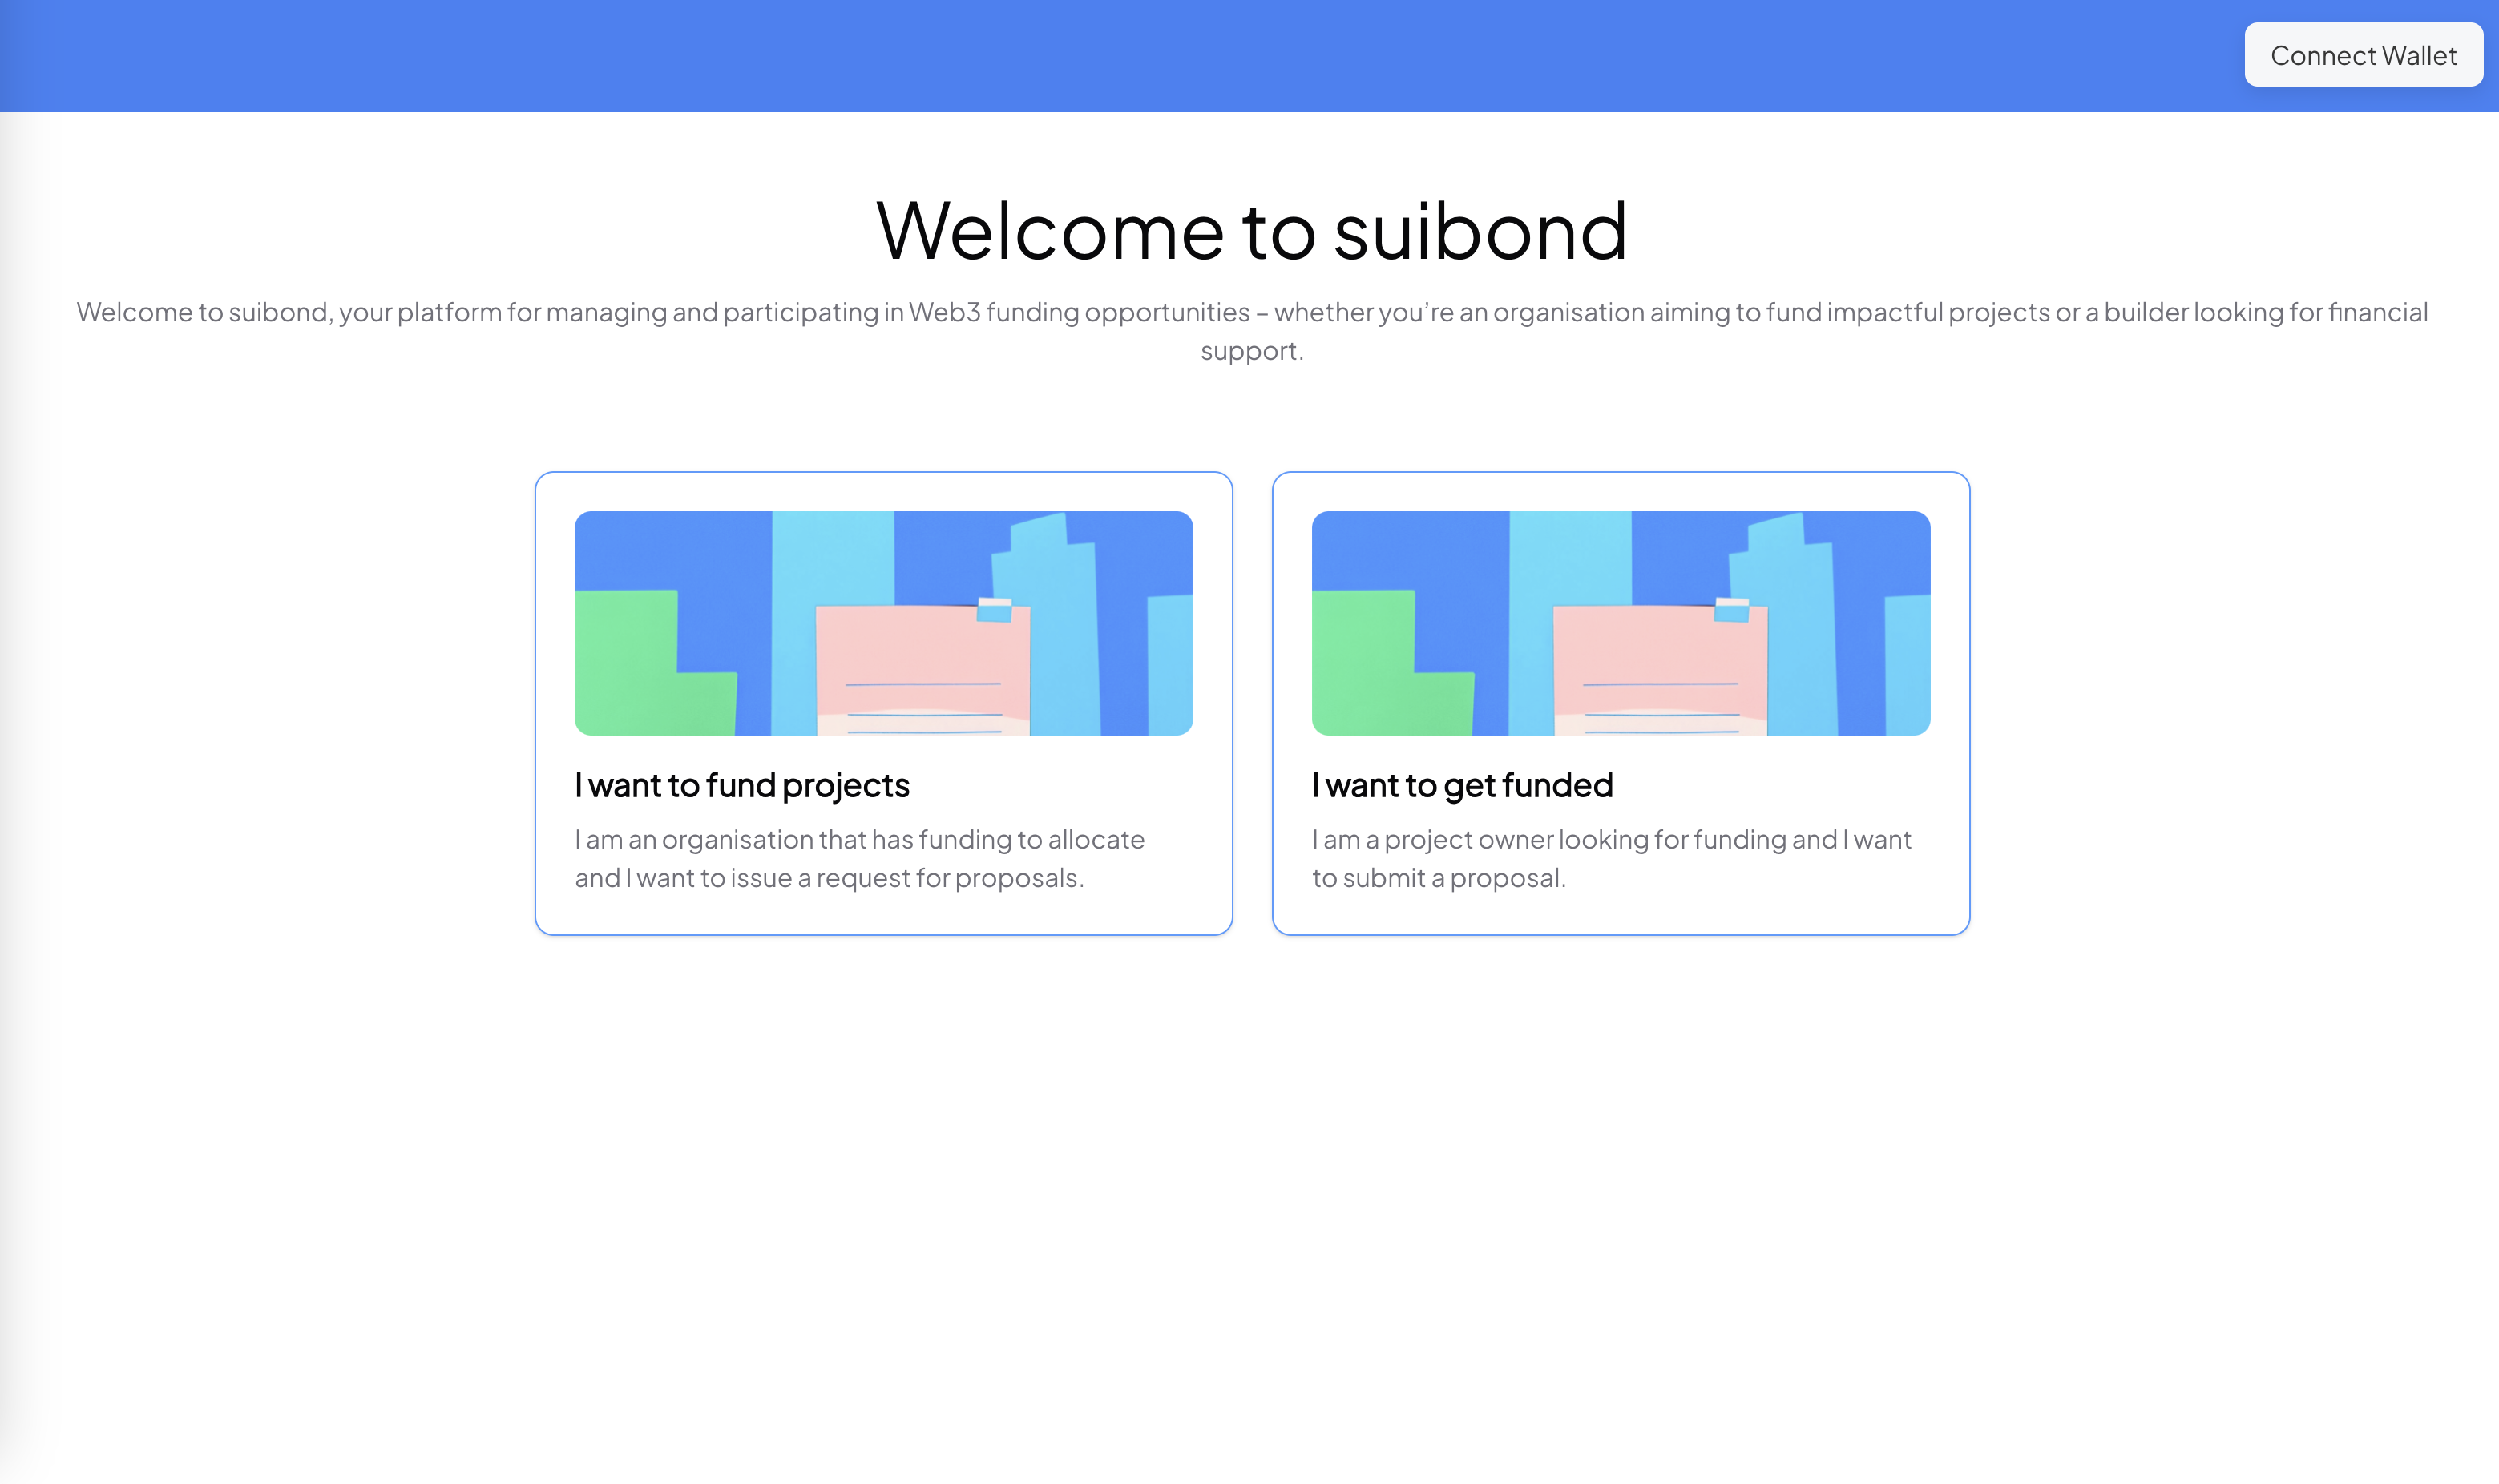
\includegraphics[scale=0.1]{suibond.png}}
\caption{This shows the suibond application.}
\label{fig}
\end{figure}


\section*{Acknowledgment}

We thank Eugene and Matthew for review and contributions.

\begin{thebibliography}{00}
\bibitem{b1} G. Eason, B. Noble, and I. N. Sneddon, ``On certain integrals of Lipschitz-Hankel type involving products of Bessel functions,'' Phil. Trans. Roy. Soc. London, vol. A247, pp. 529--551, April 1955.
\bibitem{b2} J. Clerk Maxwell, A Treatise on Electricity and Magnetism, 3rd ed., vol. 2. Oxford: Clarendon, 1892, pp.68--73.
\bibitem{b3} I. S. Jacobs and C. P. Bean, ``Fine particles, thin films and exchange anisotropy,'' in Magnetism, vol. III, G. T. Rado and H. Suhl, Eds. New York: Academic, 1963, pp. 271--350.
\bibitem{b4} K. Elissa, ``Title of paper if known,'' unpublished.
\bibitem{b5} R. Nicole, ``Title of paper with only first word capitalized,'' J. Name Stand. Abbrev., in press.
\bibitem{b6} Y. Yorozu, M. Hirano, K. Oka, and Y. Tagawa, ``Electron spectroscopy studies on magneto-optical media and plastic substrate interface,'' IEEE Transl. J. Magn. Japan, vol. 2, pp. 740--741, August 1987 [Digests 9th Annual Conf. Magnetics Japan, p. 301, 1982].
\bibitem{b7} M. Young, The Technical Writer's Handbook. Mill Valley, CA: University Science, 1989.
\bibitem{b8} D. P. Kingma and M. Welling, ``Auto-encoding variational Bayes,'' 2013, arXiv:1312.6114. [Online]. Available: https://arxiv.org/abs/1312.6114
\bibitem{b9} S. Liu, ``Wi-Fi Energy Detection Testbed (12MTC),'' 2023, gitHub repository. [Online]. Available: https://github.com/liustone99/Wi-Fi-Energy-Detection-Testbed-12MTC
\bibitem{b10} ``Treatment episode data set: discharges (TEDS-D): concatenated, 2006 to 2009.'' U.S. Department of Health and Human Services, Substance Abuse and Mental Health Services Administration, Office of Applied Studies, August, 2013, DOI:10.3886/ICPSR30122.v2
\bibitem{b11} K. Eves and J. Valasek, ``Adaptive control for singularly perturbed systems examples,'' Code Ocean, Aug. 2023. [Online]. Available: https://codeocean.com/capsule/4989235/tree
\end{thebibliography}

\end{document}
